\chapter{Evaluación de Alternativas}
\label{alternatives}

\section{Técnicas de Downsampling}

Una vez introducido el concepto de downsampling como solución al problema de visualización de series de tiempo muy densas, es necesario revisar y comparar las principales alternativas existentes.

Diversos autores han propuesto algoritmos que permiten seleccionar los puntos más representativos de una serie para facilitar su visualización. A continuación, se presenta un resumen de los métodos más relevantes:

\section{Técnicas de Downsampling}

Una vez introducido el concepto de downsampling como solución al problema de visualización de series de tiempo muy densas, es necesario revisar y comparar las principales alternativas existentes.

Diversos autores han propuesto algoritmos que permiten seleccionar los puntos más representativos de una serie para facilitar su visualización. A continuación, se presenta un resumen de los métodos implementados en la biblioteca \textit{TS Downsample}, la cual será usada durante el desarrollo de la Memoria de Título.

\subsection{Mode-Median-Bucket (MMB)} 
Divide los datos en bloques y selecciona un punto por bloque usando la moda o la mediana de los valores. Es simple y fácil de entender, pero tiende a omitir picos y valles locales relevantes~\cite{steinarsson2013downsampling}.

\paragraph{Ejemplo paso a paso:}

Supongamos la siguiente serie de 15 puntos:

\begin{center}
\begin{tabular}{|c|c|c|c|c|c|c|c|c|c|c|c|c|c|c|c|}
\hline
\textbf{Índice} & 0 & 1 & 2 & 3 & 4 & 5 & 6 & 7 & 8 & 9 & 10 & 11 & 12 & 13 & 14 \\
\hline
\textbf{Valor} & 5 & 6 & 6 & 7 & 5 & 8 & 5 & 9 & 9 & 10 & 11 & 11 & 10 & 9 & 8 \\
\hline
\end{tabular}
\end{center}


Queremos reducir a $n_{\text{out}} = 5$ puntos. \\Por lo tanto, dividimos la serie en 5 bloques de tamaño 3:

\begin{itemize}
    \item \textbf{Bloque 1 (índices 0--2)}: [5, 6, 6]  
    $\rightarrow$ Moda = 6 (ocurre 2 veces)  
    $\Rightarrow$ Se selecciona el valor \textbf{6} (índice 1)
    
    \item \textbf{Bloque 2 (índices 3--5)}: [7, 5, 8]  
    $\rightarrow$ Sin moda clara, usamos la mediana  
    Ordenado: [5, 7, 8] $\Rightarrow$ Mediana = 7  
    $\Rightarrow$ Se selecciona el valor \textbf{7} (índice 3)
    
    \item \textbf{Bloque 3 (índices 6--8)}: [5, 9, 9]  
    $\rightarrow$ Moda = 9  
    $\Rightarrow$ Se selecciona el valor \textbf{9} (índice 7)
    
    \item \textbf{Bloque 4 (índices 9--11)}: [10, 11, 11]  
    $\rightarrow$ Moda = 11  
    $\Rightarrow$ Se selecciona el valor \textbf{11} (índice 10)
    
    \item \textbf{Bloque 5 (índices 12--14)}: [10, 9, 8]  
    $\rightarrow$ Sin moda clara, usamos la mediana  
    Ordenado: [8, 9, 10] $\Rightarrow$ Mediana = 9  
    $\Rightarrow$ Se selecciona el valor \textbf{9} (índice 13)
\end{itemize}

\bigskip

\noindent \textbf{Resultado final (MMB con $n_{\text{out}} = 5$):}

\begin{center}
\begin{tabular}{|c|c|c|}
\hline
Posición resumen & Índice original & Valor \\
\hline
0 & 1 & 6 \\
1 & 3 & 7 \\
2 & 7 & 9 \\
3 & 10 & 11 \\
4 & 13 & 9 \\
\hline
\end{tabular}
\end{center}

\subsection{Min-Std-Error-Bucket (MSEB)} 
Utiliza regresión lineal para calcular el error estándar entre pares de puntos, eligiendo aquellos que minimizan la suma de errores. Produce resultados estadísticamente coherentes, pero suaviza demasiado la serie y elimina detalles visuales importantes~\cite{steinarsson2013downsampling}.

\paragraph{Ejemplo paso a paso:}

Supongamos la misma serie de 15 puntos:

\begin{center}
\begin{tabular}{|c|c|c|c|c|c|c|c|c|c|c|c|c|c|c|c|}
\hline
\textbf{Índice} & 0 & 1 & 2 & 3 & 4 & 5 & 6 & 7 & 8 & 9 & 10 & 11 & 12 & 13 & 14 \\
\hline
\textbf{Valor} & 5 & 6 & 6 & 7 & 5 & 8 & 5 & 9 & 9 & 10 & 11 & 11 & 10 & 9 & 8 \\
\hline
\end{tabular}
\end{center}

Queremos reducir a $n_{\text{out}} = 5$ puntos. \\Por lo tanto, dividimos la serie en 5 bloques de tamaño 3. Para cada bloque, seleccionamos el punto con menor error absoluto respecto a la recta entre el primer y el último punto.

\begin{itemize}
    \item \textbf{Bloque 1 (índices 0--2)}: [5, 6, 6]  
    Línea entre (0, 5) y (2, 6): pendiente \(m = \frac{6 - 5}{2 - 0} = 0.5\)  
    Valor estimado en índice 1: \( \hat{y} = 5 + 0.5 \cdot 1 = 5.5 \)  
    Errores absolutos:  
    \begin{itemize}
        \item Índice 0: $|5 - 5| = 0$
        \item Índice 1: $|6 - 5.5| = 0.5$
        \item Índice 2: $|6 - 6| = 0$
    \end{itemize}
    Mínimo error: índice \textbf{0} y \textbf{2}. Tomamos el primero: \textbf{5} (índice 0)

    \item \textbf{Bloque 2 (índices 3--5)}: [7, 5, 8]  
    Línea entre (3, 7) y (5, 8): \(m = \frac{8 - 7}{2} = 0.5\)  
    Valor estimado en índice 4: \( \hat{y} = 7 + 0.5 = 7.5 \)  
    Errores:  
    \begin{itemize}
        \item Índice 3: $|7 - 7| = 0$
        \item Índice 4: $|5 - 7.5| = 2.5$
        \item Índice 5: $|8 - 8| = 0$
    \end{itemize}
    Mínimo error: índice \textbf{3} y \textbf{5}. Tomamos el primero: \textbf{7} (índice 3)

    \item \textbf{Bloque 3 (índices 6--8)}: [5, 9, 9]  
    Línea entre (6, 5) y (8, 9): \(m = \frac{9 - 5}{2} = 2\)  
    Valor estimado en índice 7: \( \hat{y} = 5 + 2 = 7 \)  
    Errores:  
    \begin{itemize}
        \item Índice 6: $|5 - 5| = 0$
        \item Índice 7: $|9 - 7| = 2$
        \item Índice 8: $|9 - 9| = 0$
    \end{itemize}
    Mínimo error: índice \textbf{6} y \textbf{8}. Tomamos el primero: \textbf{5} (índice 6)

    \item \textbf{Bloque 4 (índices 9--11)}: [10, 11, 11]  
    Línea entre (9, 10) y (11, 11): \(m = \frac{11 - 10}{2} = 0.5\)  
    Valor estimado en índice 10: \( \hat{y} = 10 + 0.5 = 10.5 \)  
    Errores:  
    \begin{itemize}
        \item Índice 9: $|10 - 10| = 0$
        \item Índice 10: $|11 - 10.5| = 0.5$
        \item Índice 11: $|11 - 11| = 0$
    \end{itemize}
    Mínimo error: índice \textbf{9} y \textbf{11}. Tomamos el primero: \textbf{10} (índice 9)

    \item \textbf{Bloque 5 (índices 12--14)}: [10, 9, 8]  
    Línea entre (12, 10) y (14, 8): \(m = \frac{8 - 10}{2} = -1\)  
    Valor estimado en índice 13: \( \hat{y} = 10 + (-1) = 9 \)  
    Errores:  
    \begin{itemize}
        \item Índice 12: $|10 - 10| = 0$
        \item Índice 13: $|9 - 9| = 0$
        \item Índice 14: $|8 - 8| = 0$
    \end{itemize}
    Todos tienen error 0. Tomamos el primero: \textbf{10} (índice 12)
\end{itemize}

\bigskip

\noindent \textbf{Resultado final (MSEB con $n_{\text{out}} = 5$):}

\begin{center}
\begin{tabular}{|c|c|c|}
\hline
Posición resumen & Índice original & Valor \\
\hline
0 & 0 & 5 \\
1 & 3 & 7 \\
2 & 6 & 5 \\
3 & 9 & 10 \\
4 & 12 & 10 \\
\hline
\end{tabular}
\end{center}


\subsection{Longest-Line-Bucket (LLB)} 
Similar a MSEB, pero en lugar de minimizar el error estándar, selecciona el punto intermedio que, junto con el inicio y el final del bloque, forma la línea de mayor longitud. Esta técnica es útil para preservar picos extremos y fluctuaciones relevantes~\cite{steinarsson2013downsampling}.

\paragraph{Ejemplo paso a paso:}

Utilizamos la misma serie de 15 puntos:

\begin{center}
\begin{tabular}{|c|c|c|c|c|c|c|c|c|c|c|c|c|c|c|c|}
\hline
\textbf{Índice} & 0 & 1 & 2 & 3 & 4 & 5 & 6 & 7 & 8 & 9 & 10 & 11 & 12 & 13 & 14 \\
\hline
\textbf{Valor} & 5 & 6 & 6 & 7 & 5 & 8 & 5 & 9 & 9 & 10 & 11 & 11 & 10 & 9 & 8 \\
\hline
\end{tabular}
\end{center}

Queremos reducir a $n_{\text{out}} = 5$ puntos. \\Dividimos la serie en 5 bloques de tamaño 3. Para cada bloque, se calcula la distancia euclidiana entre los pares (inicio-intermedio) y (intermedio-fin), y se selecciona el punto con mayor suma de longitudes.

\begin{itemize}
    \item \textbf{Bloque 1 (índices 0--2)}: [5, 6, 6]
    \begin{itemize}
        \item Línea (0,5)-(1,6)-(2,6):
        \begin{itemize}
            \item Distancia (0,5)-(1,6): $\sqrt{1^2 + 1^2} \approx 1.41$
            \item Distancia (1,6)-(2,6): $\sqrt{1^2 + 0^2} = 1$
            \item Suma total: 2.41
        \end{itemize}
        \item Punto medio: \textbf{1} → Valor: \textbf{6}
    \end{itemize}

    \item \textbf{Bloque 2 (índices 3--5)}: [7, 5, 8]
    \begin{itemize}
        \item Línea (3,7)-(4,5)-(5,8):
        \begin{itemize}
            \item Distancia (3,7)-(4,5): $\sqrt{1^2 + 2^2} \approx 2.24$
            \item Distancia (4,5)-(5,8): $\sqrt{1^2 + 3^2} \approx 3.16$
            \item Suma total: 5.40
        \end{itemize}
        \item Punto medio: \textbf{4} → Valor: \textbf{5}
    \end{itemize}

    \item \textbf{Bloque 3 (índices 6--8)}: [5, 9, 9]
    \begin{itemize}
        \item Línea (6,5)-(7,9)-(8,9):
        \begin{itemize}
            \item Distancia (6,5)-(7,9): $\sqrt{1^2 + 4^2} \approx 4.12$
            \item Distancia (7,9)-(8,9): $1$
            \item Suma total: 5.12
        \end{itemize}
        \item Punto medio: \textbf{7} → Valor: \textbf{9}
    \end{itemize}

    \item \textbf{Bloque 4 (índices 9--11)}: [10, 11, 11]
    \begin{itemize}
        \item Línea (9,10)-(10,11)-(11,11):
        \begin{itemize}
            \item Distancia (9,10)-(10,11): $\sqrt{1^2 + 1^2} \approx 1.41$
            \item Distancia (10,11)-(11,11): $1$
            \item Suma total: 2.41
        \end{itemize}
        \item Punto medio: \textbf{10} → Valor: \textbf{11}
    \end{itemize}

    \item \textbf{Bloque 5 (índices 12--14)}: [10, 9, 8]
    \begin{itemize}
        \item Línea (12,10)-(13,9)-(14,8):
        \begin{itemize}
            \item Distancia (12,10)-(13,9): $\sqrt{1^2 + 1^2} \approx 1.41$
            \item Distancia (13,9)-(14,8): $\sqrt{1^2 + 1^2} \approx 1.41$
            \item Suma total: 2.83
        \end{itemize}
        \item Punto medio: \textbf{13} → Valor: \textbf{9}
    \end{itemize}
\end{itemize}

\bigskip

\noindent \textbf{Resultado final (LLB con $n_{\text{out}} = 5$):}

\begin{center}
\begin{tabular}{|c|c|c|}
\hline
Posición resumen & Índice original & Valor \\
\hline
0 & 1 & 6 \\
1 & 4 & 5 \\
2 & 7 & 9 \\
3 & 10 & 11 \\
4 & 13 & 9 \\
\hline
\end{tabular}
\end{center}

\subsection{Largest-Triangle-Three-Buckets (LTTB)} 
Divide los datos en grupos de tres bloques consecutivos. En cada paso, selecciona el punto intermedio del bloque central que forma el triángulo de mayor área con los puntos de los bloques anterior y posterior. Preserva bien la forma general del gráfico y es eficiente computacionalmente~\cite{steinarsson2013downsampling}.

\paragraph{Ejemplo paso a paso:}

Usamos la misma serie de 15 puntos:

\begin{center}
\begin{tabular}{|c|c|c|c|c|c|c|c|c|c|c|c|c|c|c|c|}
\hline
\textbf{Índice} & 0 & 1 & 2 & 3 & 4 & 5 & 6 & 7 & 8 & 9 & 10 & 11 & 12 & 13 & 14 \\
\hline
\textbf{Valor} & 5 & 6 & 6 & 7 & 5 & 8 & 5 & 9 & 9 & 10 & 11 & 11 & 10 & 9 & 8 \\
\hline
\end{tabular}
\end{center}

Seleccionamos 5 puntos: el primero (índice 0), tres intermedios, y el último (índice 14).

Para elegir los 3 intermedios, aplicamos LTTB en 3 iteraciones:

\begin{itemize}
    \item \textbf{Paso 1 (Bloques 0--4)}:
    \begin{itemize}
        \item Punto anterior: A = (0,5)
        \item Candidatos: (1,6), (2,6), (3,7)
        \item Centroide siguiente bloque: Promedio de (4,5), (5,8), (6,5): centro = (5,6)
        \item Área de triángulos:
        \begin{itemize}
            \item A-(1,6)-(5,6) = 2.0
            \item A-(2,6)-(5,6) = 2.5
            \item A-(3,7)-(5,6) = 4.0
        \end{itemize}
        \item Mayor área: 4.0 → Se elige \textbf{(3,7)}
    \end{itemize}

    \item \textbf{Paso 2 (Bloques 4--8)}:
    \begin{itemize}
        \item Punto anterior: A = (3,7)
        \item Candidatos: (4,5), (5,8), (6,5)
        \item Centroide siguiente bloque: Promedio de (7,9), (8,9), (9,10): centro = (8,9.3)
        \item Área de triángulos:
        \begin{itemize}
            \item A-(4,5)-(8,9.3) ≈ 2.9
            \item A-(5,8)-(8,9.3) ≈ 1.65
            \item A-(6,5)-(8,9.3) ≈ 4.6
        \end{itemize}
        \item Mayor área: ≈ 4.6 → Se elige \textbf{(6,5)}
    \end{itemize}

    \item \textbf{Paso 3 (Bloques 8--13)}:
    \begin{itemize}
        \item Punto anterior: A = (6,5)
        \item Candidatos: (7,9), (8,9), (9,10), (10,11), (11,11)
        \item Centroide siguiente bloque: Promedio de (12,10), (13,9), (14,8): centro = (13,9)
        \item Áreas:
        \begin{itemize}
            \item A-(7,9)-(13,9) ≈ 12.0
            \item A-(8,9)-(13,9) ≈ 13.0
            \item A-(9,10)-(13,9) ≈ 15.0
            \item A-(10,11)-(13,9) ≈ 17.0
            \item A-(11,11)-(13,9) ≈ 15.0
        \end{itemize}
        \item Mayor área: 17.0 → Se elige \textbf{(10,11)}
    \end{itemize}
\end{itemize}

\bigskip

\noindent \textbf{Resultado final (LTTB con $n_{\text{out}} = 5$):}

\begin{center}
\begin{tabular}{|c|c|c|}
\hline
Posición resumen & Índice original & Valor \\
\hline
0 & 0 & 5 \\
1 & 3 & 7 \\
2 & 6 & 5 \\
3 & 10 & 11 \\
4 & 14 & 8 \\
\hline
\end{tabular}
\end{center}

\subsection{Largest-Triangle-Dynamic (LTD)} 
Variante de LTTB que adapta dinámicamente el tamaño de los bloques según la variación local de los datos. Busca mantener más puntos en regiones con alta variabilidad y menos en regiones estables~\cite{steinarsson2013downsampling}.

\paragraph{Ejemplo paso a paso:}

Serie original:

\begin{center}
\begin{tabular}{|c|c|c|c|c|c|c|c|c|c|c|c|c|c|c|c|}
\hline
\textbf{Índice} & 0 & 1 & 2 & 3 & 4 & 5 & 6 & 7 & 8 & 9 & 10 & 11 & 12 & 13 & 14 \\
\hline
\textbf{Valor} & 5 & 6 & 6 & 7 & 5 & 8 & 5 & 9 & 9 & 10 & 11 & 11 & 10 & 9 & 8 \\
\hline
\end{tabular}
\end{center}

Queremos reducir a \(n_{\text{out}} = 5\) puntos, manteniendo:

- El primer punto (índice 0)
- El último punto (índice 14)
- 3 puntos intermedios seleccionados con bloques adaptativos

\bigskip

\noindent Para determinar la variación local usamos una métrica simple: \textbf{rango} (máx - mín) en bloques consecutivos. Esto nos ayuda a redistribuir los puntos proporcionalmente.

\begin{itemize}
    \item Bloque 1: índices 1–5 → [6,6,7,5,8] → rango = 8 - 5 = 3
    \item Bloque 2: índices 6–10 → [5,9,9,10,11] → rango = 11 - 5 = 6
    \item Bloque 3: índices 11–13 → [11,10,9] → rango = 11 - 9 = 2
\end{itemize}

Total rango: \(3 + 6 + 2 = 11\)

Distribuimos los 3 puntos intermedios proporcionalmente:

\begin{itemize}
    \item Bloque 1: \(3 \times \frac{3}{11} ≈ 0.82\) \Rightarrow 1 punto
    \item Bloque 2: \(3 \times \frac{6}{11} ≈ 1.64\) \Rightarrow 2 puntos
    \item Bloque 3: \(3 \times \frac{2}{11} ≈ 0.55\) \Rightarrow 0 puntos (pero tomamos 1 de aquí para no desperdiciar rango)
\end{itemize}

\textbf{Puntos seleccionados:}

\begin{itemize}
    \item \textbf{Bloque 1 (1–5)}: usamos LTTB con anterior (0,5), siguiente centroide = (6,7)
    
    Candidatos: (1,6), (2,6), (3,7), (4,5), (5,8)  
    Mayor área con triángulo: → (3,7)
    
    \item \textbf{Bloque 2 (6–10)}: anterior = (3,7), siguiente centroide = (11,10)
    
    Candidatos: (6,5), (7,9), (8,9), (9,10), (10,11)  
    Dos mayores áreas → seleccionamos (7,9) y (10,11)
    
    \item \textbf{Bloque 3 (11–13)}: no se asignó punto originalmente, pero por cobertura tomamos el más representativo
    
    Máximo local: (11,11)
\end{itemize}

\bigskip

\noindent \textbf{Resultado final (LTD con $n_{\text{out}} = 5$):}

\begin{center}
\begin{tabular}{|c|c|c|}
\hline
Posición resumen & Índice original & Valor \\
\hline
0 & 0 & 5 \\
1 & 3 & 7 \\
2 & 7 & 9 \\
3 & 10 & 11 \\
4 & 14 & 8 \\
\hline
\end{tabular}
\end{center}

\subsection{MinMaxLTTB} 
Propuesto por Van Der Donckt {\it et al.}~\cite{vanderdonckt2023minmaxlttb}, este algoritmo mejora la eficiencia del método LTTB aplicando una preselección vertical de puntos significativos mediante mínimos y máximos por bloque (algoritmo MinMax), seguido de la selección final con LTTB sobre ese conjunto reducido. Esto permite una aceleración sustancial sin sacrificar la fidelidad visual.

\paragraph{Ejemplo paso a paso:}

Usamos la misma serie de 15 puntos:

\begin{center}
\begin{tabular}{|c|c|c|c|c|c|c|c|c|c|c|c|c|c|c|c|}
\hline
\textbf{Índice} & 0 & 1 & 2 & 3 & 4 & 5 & 6 & 7 & 8 & 9 & 10 & 11 & 12 & 13 & 14 \\
\hline
\textbf{Valor} & 5 & 6 & 6 & 7 & 5 & 8 & 5 & 9 & 9 & 10 & 11 & 11 & 10 & 9 & 8 \\
\hline
\end{tabular}
\end{center}

Queremos reducir a $n_{\text{out}} = 5$ puntos. Por lo tanto, necesitamos:

\begin{itemize}
    \item 1er punto (siempre se incluye): índice 0
    \item Último punto (también se incluye): índice 14
    \item 3 puntos intermedios: se obtienen con MinMax + LTTB
\end{itemize}

\bigskip

\textbf{Paso 1: Preselección con MinMax}

Dividimos los puntos intermedios (índices 1 a 13) en 3 bloques:

\begin{itemize}
    \item \textbf{Bloque 1 (índices 1--4)}: valores [6, 6, 7, 5]  
    $\rightarrow$ Mínimo: (4, 5), Máximo: (3, 7)
    
    \item \textbf{Bloque 2 (índices 5--8)}: valores [8, 5, 9, 9]  
    $\rightarrow$ Mínimo: (6, 5), Máximo: (7, 9)
    
    \item \textbf{Bloque 3 (índices 9--13)}: valores [10, 11, 11, 10, 9]  
    $\rightarrow$ Mínimo: (13, 9), Máximo: (10, 11)
\end{itemize}

\noindent Candidatos seleccionados por MinMax (ordenados por índice):

\[
(3,7),\ (4,5),\ (6,5),\ (7,9),\ (10,11),\ (13,9)
\]

\bigskip

\textbf{Paso 2: Aplicar LTTB sobre los puntos candidatos}

LTTB se aplica para seleccionar 3 puntos intermedios entre:

\[
(0,5) \quad \text{(inicio)}, \quad \text{candidatos MinMax}, \quad (14,8) \quad \text{(fin)}
\]

Se agrupan los puntos candidatos en 3 bloques:

\begin{itemize}
    \item \textbf{Bloque 1}: [(3,7), (4,5)]  
    $\rightarrow$ Triángulo con base (0,5) y siguiente centro = (6,5)  
    $\Rightarrow$ Área de (3,7) es mayor que la de (4,5)  
    $\Rightarrow$ Se selecciona (3,7)

    \item \textbf{Bloque 2}: [(6,5), (7,9)]  
    $\rightarrow$ Triángulo con base (3,7) y siguiente centro = (10,11)  
    $\Rightarrow$ Área de (7,9) es mayor que la de (6,5)  
    $\Rightarrow$ Se selecciona (7,9)

    \item \textbf{Bloque 3}: [(10,11), (13,9)]  
    $\rightarrow$ Triángulo con base (7,9) y siguiente punto final = (14,8)  
    $\Rightarrow$ Área de (10,11) es mayor que la de (13,9)  
    $\Rightarrow$ Se selecciona (10,11)
\end{itemize}

\bigskip

\noindent \textbf{Resultado final (MinMaxLTTB con $n_{\text{out}} = 5$):}

\begin{center}
\begin{tabular}{|c|c|c|}
\hline
Posición resumen & Índice original & Valor \\
\hline
0 & 0 & 5 \\
1 & 3 & 7 \\
2 & 7 & 9 \\
3 & 10 & 11 \\
4 & 14 & 8 \\
\hline
\end{tabular}
\end{center}


Dado el enfoque de este trabajo, se seleccionó principalmente el uso del algoritmo \textbf{MinMaxLTTB}. Esta decisión se fundamenta en varios factores: en primer lugar, el algoritmo ha sido propuesto por los mismos autores que desarrollaron la biblioteca \texttt{tsdownsample}, lo que garantiza una implementación de referencia optimizada y bien documentada. Además, MinMaxLTTB presenta un excelente equilibrio entre rendimiento y fidelidad visual, al combinar una reducción sustancial en el tiempo de cómputo con una buena preservación de la forma general de la serie de tiempo.

Como complemento para el análisis comparativo, también se utilizará el algoritmo \textbf{LTTB}, ya que es ampliamente citado en la literatura como una opción base eficiente, y su comparación directa con MinMaxLTTB permite observar el impacto de la estrategia de preselección aplicada por los autores.

\newpage
\section{Estructuras de Datos Compactas}

Las estructuras de datos compactas ofrecen una alternativa más eficiente en espacio frente a las estructuras clásicas basadas en punteros, especialmente cuando se busca representar grandes volúmenes de datos. Estas estructuras permiten codificar secuencias numéricas utilizando una menor cantidad de bits por elemento, sin pérdida de información y manteniendo la posibilidad de acceso eficiente a los datos.

En la literatura existen bibliotecas que implementan estas estructuras. En particular, utilizaremos la biblioteca \texttt{sdsl4py}\cite{sdsl4py2024}, un conjunto de bindings en Python para la Succinct Data Structure Library (SDSL)\cite{gbmp2014sea}, que permite acceder a múltiples representaciones compactas desde Python. A continuación se presentan las estructuras de datos compactas que fueron consideradas en esta memoria de título:

\begin{enumerate}
    \item \textbf{Tipos de Codificación}
        \begin{enumerate}
            \item \texttt{Elias-Gamma}:
            Eficiente para valores pequeños. No puede codificar ceros.
            \begin{enumerate}
                \item Codificación:
                \begin{itemize}
                    \item Para cada \(x_i > 0\):
                        \begin{itemize}
                            \item \(\text{bin}(x_i)\)
                            \item \(\mathcal{L} = \lfloor \log_2 x_i \rfloor + 1\)
                            \item Prefijo: \(\mathcal{L} - 1\) ceros + binario
                        \end{itemize}
                \end{itemize}
                \item Decodificación:
                \begin{itemize}
                    \item Contar ceros → leer \(\mathcal{L}\) bits → convertir a entero
                \end{itemize}
            \end{enumerate}
            \begin{figure}
                \centering
                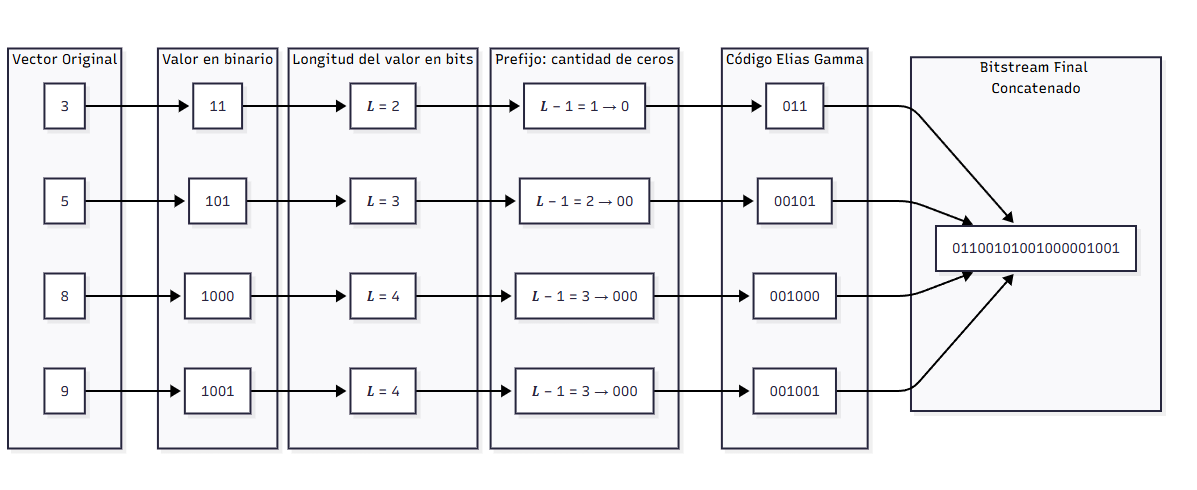
\includegraphics[width=0.9\linewidth]{alternatives/images/enc_vector_elias_gamma.png}
                \caption[Ejemplo \textit{Elias Gamma}]{Diagrama paso a paso de codificación usando la codificación \textit{Elias Gamma}.}
                \label{enc_vector_elias_gamma}
            \end{figure}

            \item \texttt{Elias-Delta}:
            Mejor que Elias-Gamma para valores grandes.
            \begin{enumerate}
                \item Codificación:
                \begin{itemize}
                    \item Para cada \(x_i > 0\):
                        \begin{itemize}
                            \item \(\mathcal{L} = \lfloor \log_2 x_i \rfloor + 1\)
                            \item Codificar \(\mathcal{L}\) con Elias-Gamma
                            \item Concatenar con los bits de \(x_i\) excepto el más significativo
                        \end{itemize}
                \end{itemize}
                \item Decodificación:
                \begin{itemize}
                    \item Decodificar \(\mathcal{L}\) con Elias-Gamma → leer \(\mathcal{L} - 1\) bits → anteponer 1
                \end{itemize}
            \end{enumerate}
            \begin{figure}[H]
                \centering
                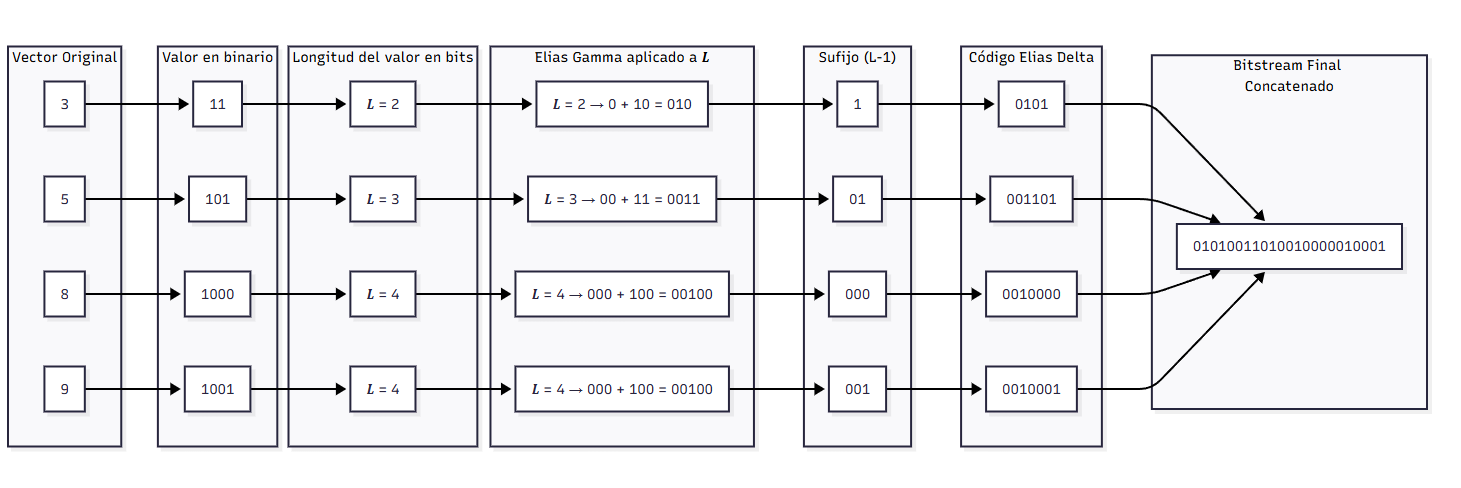
\includegraphics[width=0.9\linewidth]{alternatives/images/enc_vector_elias_delta.png}
                \caption[Ejemplo \textit{Elias Delta}]{Diagrama paso a paso de codificación \textit{Elias Delta}.}
                \label{enc_vector_elias_delta}
            \end{figure}

            \item \texttt{Fibonacci}:
            Basado en representación de Zeckendorf. Libre de prefijos.
            \begin{enumerate}
                \item Codificación:
                \begin{itemize}
                    \item Representar como suma de términos Fibonacci no consecutivos
                    \item Bitmask con 1s donde se usa el término
                    \item Agregar un bit 1 final como terminador
                \end{itemize}
                \item Decodificación:
                \begin{itemize}
                    \item Leer hasta encontrar 11 → sumar términos con 1
                \end{itemize}
            \end{enumerate}
            \begin{figure}[H]
                \centering
                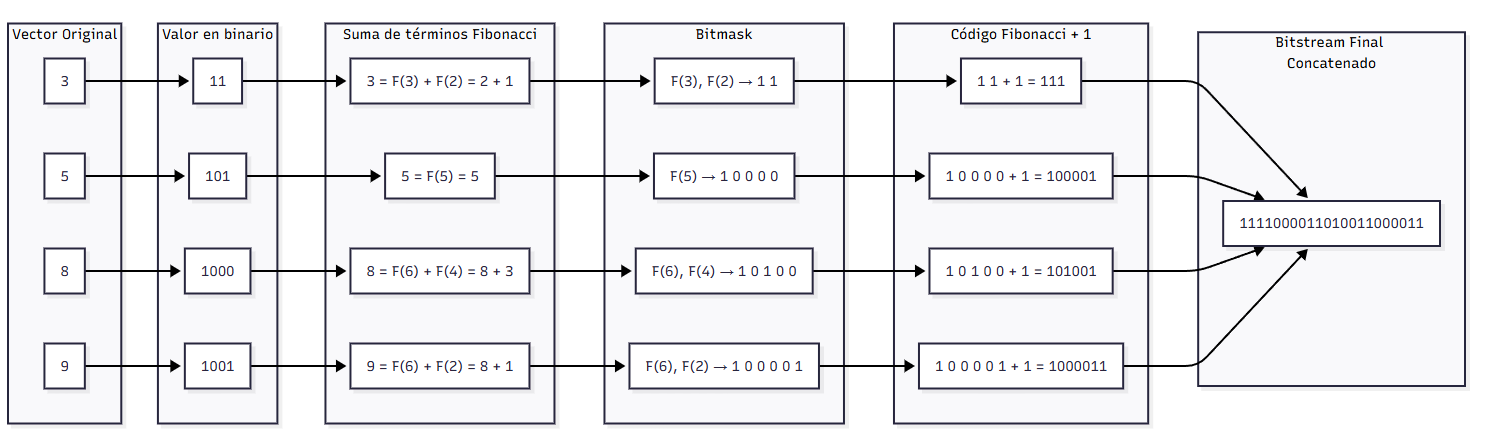
\includegraphics[width=0.9\linewidth]{alternatives/images/enc_vector_fibonacci.png}
                \caption[Ejemplo \textit{Fibonacci}]{Diagrama paso a paso de codificación \textit{Fibonacci}.}
                \label{enc_vector_fibonacci}
            \end{figure}

            \item \texttt{Comma-2}:
            Usa base \(b = 2^{t_{\text{width}}} - 1\). Cada dígito tiene ancho fijo y se finaliza con un terminador \(b\).
            \begin{enumerate}
                \item Codificación:
                \begin{itemize}
                    \item Convertir \(x_i\) a base \(b\), codificar cada dígito en \(t_{\text{width}}\) bits
                    \item Añadir dígito terminador (\(b\))
                \end{itemize}
                \item Decodificación:
                \begin{itemize}
                    \item Leer bloques de \(t_{\text{width}}\) bits → detener en terminador
                \end{itemize}
            \end{enumerate}
            \begin{figure}[H]
                \centering
                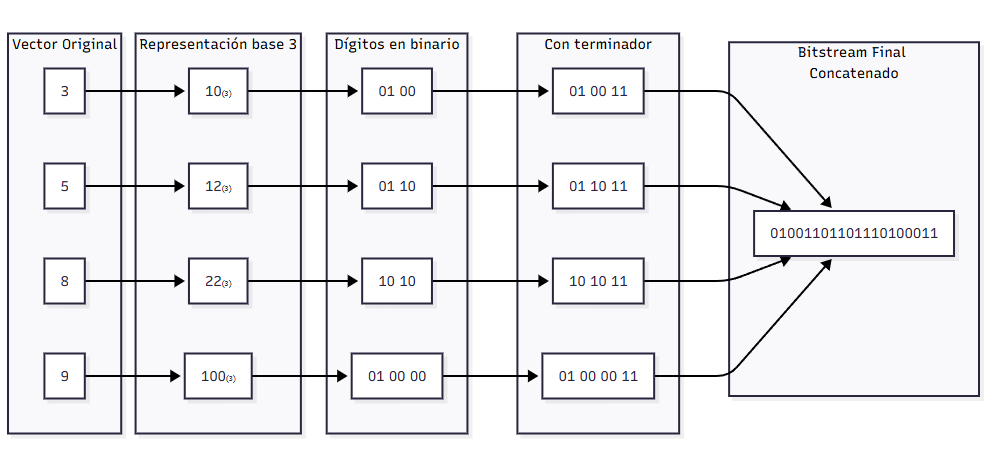
\includegraphics[width=0.9\linewidth]{alternatives/images/enc_vector_comma.png}
                \caption[Ejemplo \textit{Comma 2}]{Diagrama paso a paso de codificación por comas binarias (base \(2^2 - 1 = 3\)).}
                \label{enc_vector_comma_2}
            \end{figure}
        \end{enumerate}

    \item \textbf{Tipos De Vector}
        \begin{enumerate}
            \item \texttt{enc\_vector}:
            Codifica todos los valores de forma secuencial usando un método (Elias-Gamma, Delta, Fibonacci, Comma-2) sin estructura de acceso rápido. Compacto, pero acceso lineal.

            \item \texttt{vlc\_vector}:
            Añade acceso eficiente mediante muestreo cada \(t_{\text{dens}}\) elementos. Guarda un índice de posiciones bitstream llamado \texttt{m\_sample\_pointer}.

            \begin{itemize}
                \item Soporta las mismas codificaciones: Elias-Gamma, Elias-Delta, Fibonacci, Comma-2
                \item Acceso:
                    \begin{itemize}
                        \item Determinar muestra previa (\(j = \lfloor i / t_{\text{dens}} \rfloor\))
                        \item Decodificar desde posición \(\texttt{m\_sample\_pointer}[j]\) hasta llegar a \(x_i\)
                    \end{itemize}
            \end{itemize}

            \begin{figure}[H]
                \centering
                \makebox[\textwidth][c]{%
                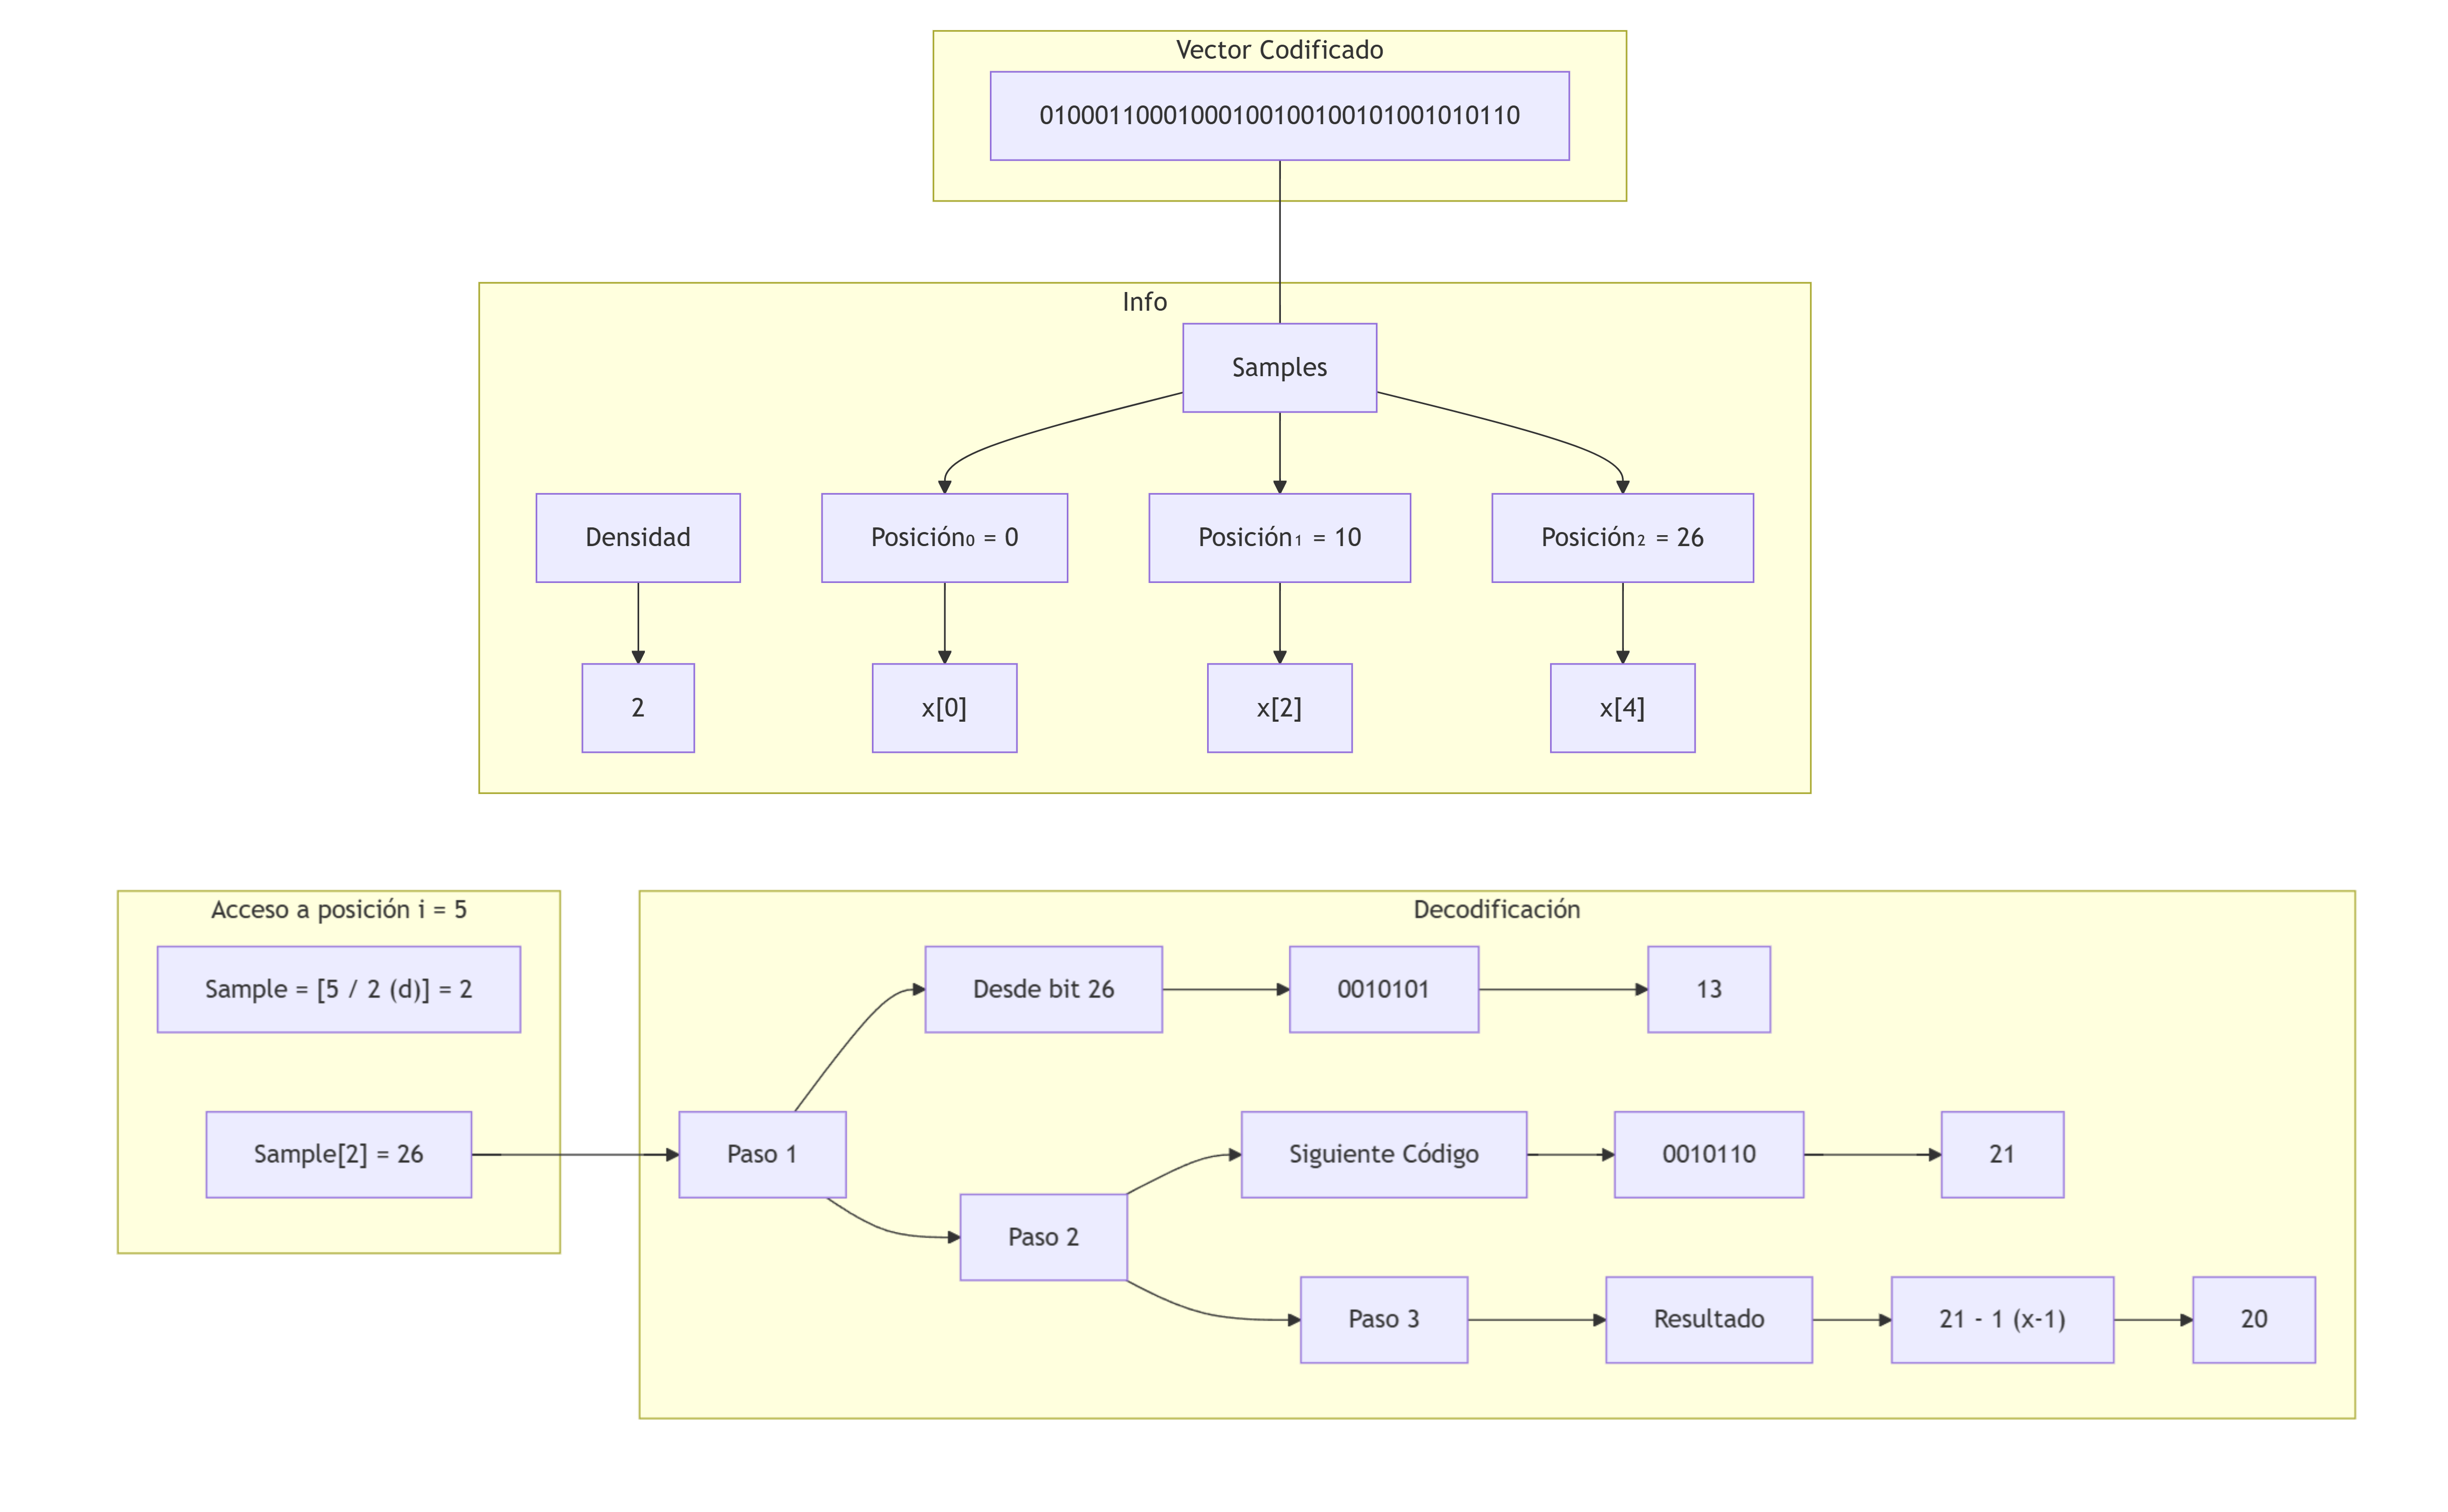
\includegraphics[width=1\textwidth]{alternatives/images/vlc_vector.png}}
                \caption[Ejemplo \texttt{vlc\_vector}]{Ejemplo de acceso a la posición $i$ en un vector \textit{VLC}.}
                \label{dac_vector}
            \end{figure}

            \item \texttt{dac\_vector}:
            Estructura basada en \textit{Directly Addressable Codes} (DAC), que permite representar enteros de forma escalonada para equilibrar compresión y velocidad de acceso. Esta técnica es especialmente útil para secuencias con valores muy dispares (alta varianza).
            \begin{enumerate}
                \item Codificación:
                \begin{itemize}
                    \item Se representa cada entero \( x_i > 0 \) en binario.
                    \item El número binario se divide en bloques de ancho fijo \( t_{\text{width}} \) comenzando desde el bit más significativo. Cada bloque se guarda en un nivel distinto.
                    \item Se construye un vector de bits por nivel llamado \texttt{bit\_vector}, donde cada bit indica si el valor continúa en el siguiente nivel (1) o si termina (0).
                    \item Para cada nivel, se almacenan:
                    \begin{itemize}
                        \item Los bloques correspondientes a ese nivel (\texttt{data\_level[i]})
                        \item El vector de continuidad (\texttt{bit\_vector[i]})
                        \item Una estructura auxiliar de acceso tipo \texttt{rank\_support} para contar cuántos valores han continuado hasta cierta posición.
                    \end{itemize}
                \end{itemize}

                \item Decodificación:
                \begin{itemize}
                    \item Se comienza en el nivel 0, leyendo el bloque de datos y el bit de continuidad.
                    \item Si el bit es 1 (continuar), se calcula el índice correspondiente en el siguiente nivel usando una operación de \texttt{rank} sobre el \texttt{bit\_vector}.
                    \item Este proceso se repite nivel por nivel, concatenando los bloques binarios hasta encontrar un bit de continuación 0.
                    \item El número binario resultante se interpreta como el valor original \(x_i\).
                \end{itemize}

                \item Ventajas:
                \begin{itemize}
                    \item Permite acceso directo a cualquier elemento en tiempo logarítmico con pocos saltos de nivel.
                    \item Se adapta bien a datos con enteros muy variados, manteniendo buen rendimiento de compresión.
                    \item La estructura escalonada evita decodificar todo el bitstream secuencialmente.
                \end{itemize}
            \end{enumerate}
            \begin{figure}[H]
                \centering
                \makebox[\textwidth][c]{%
                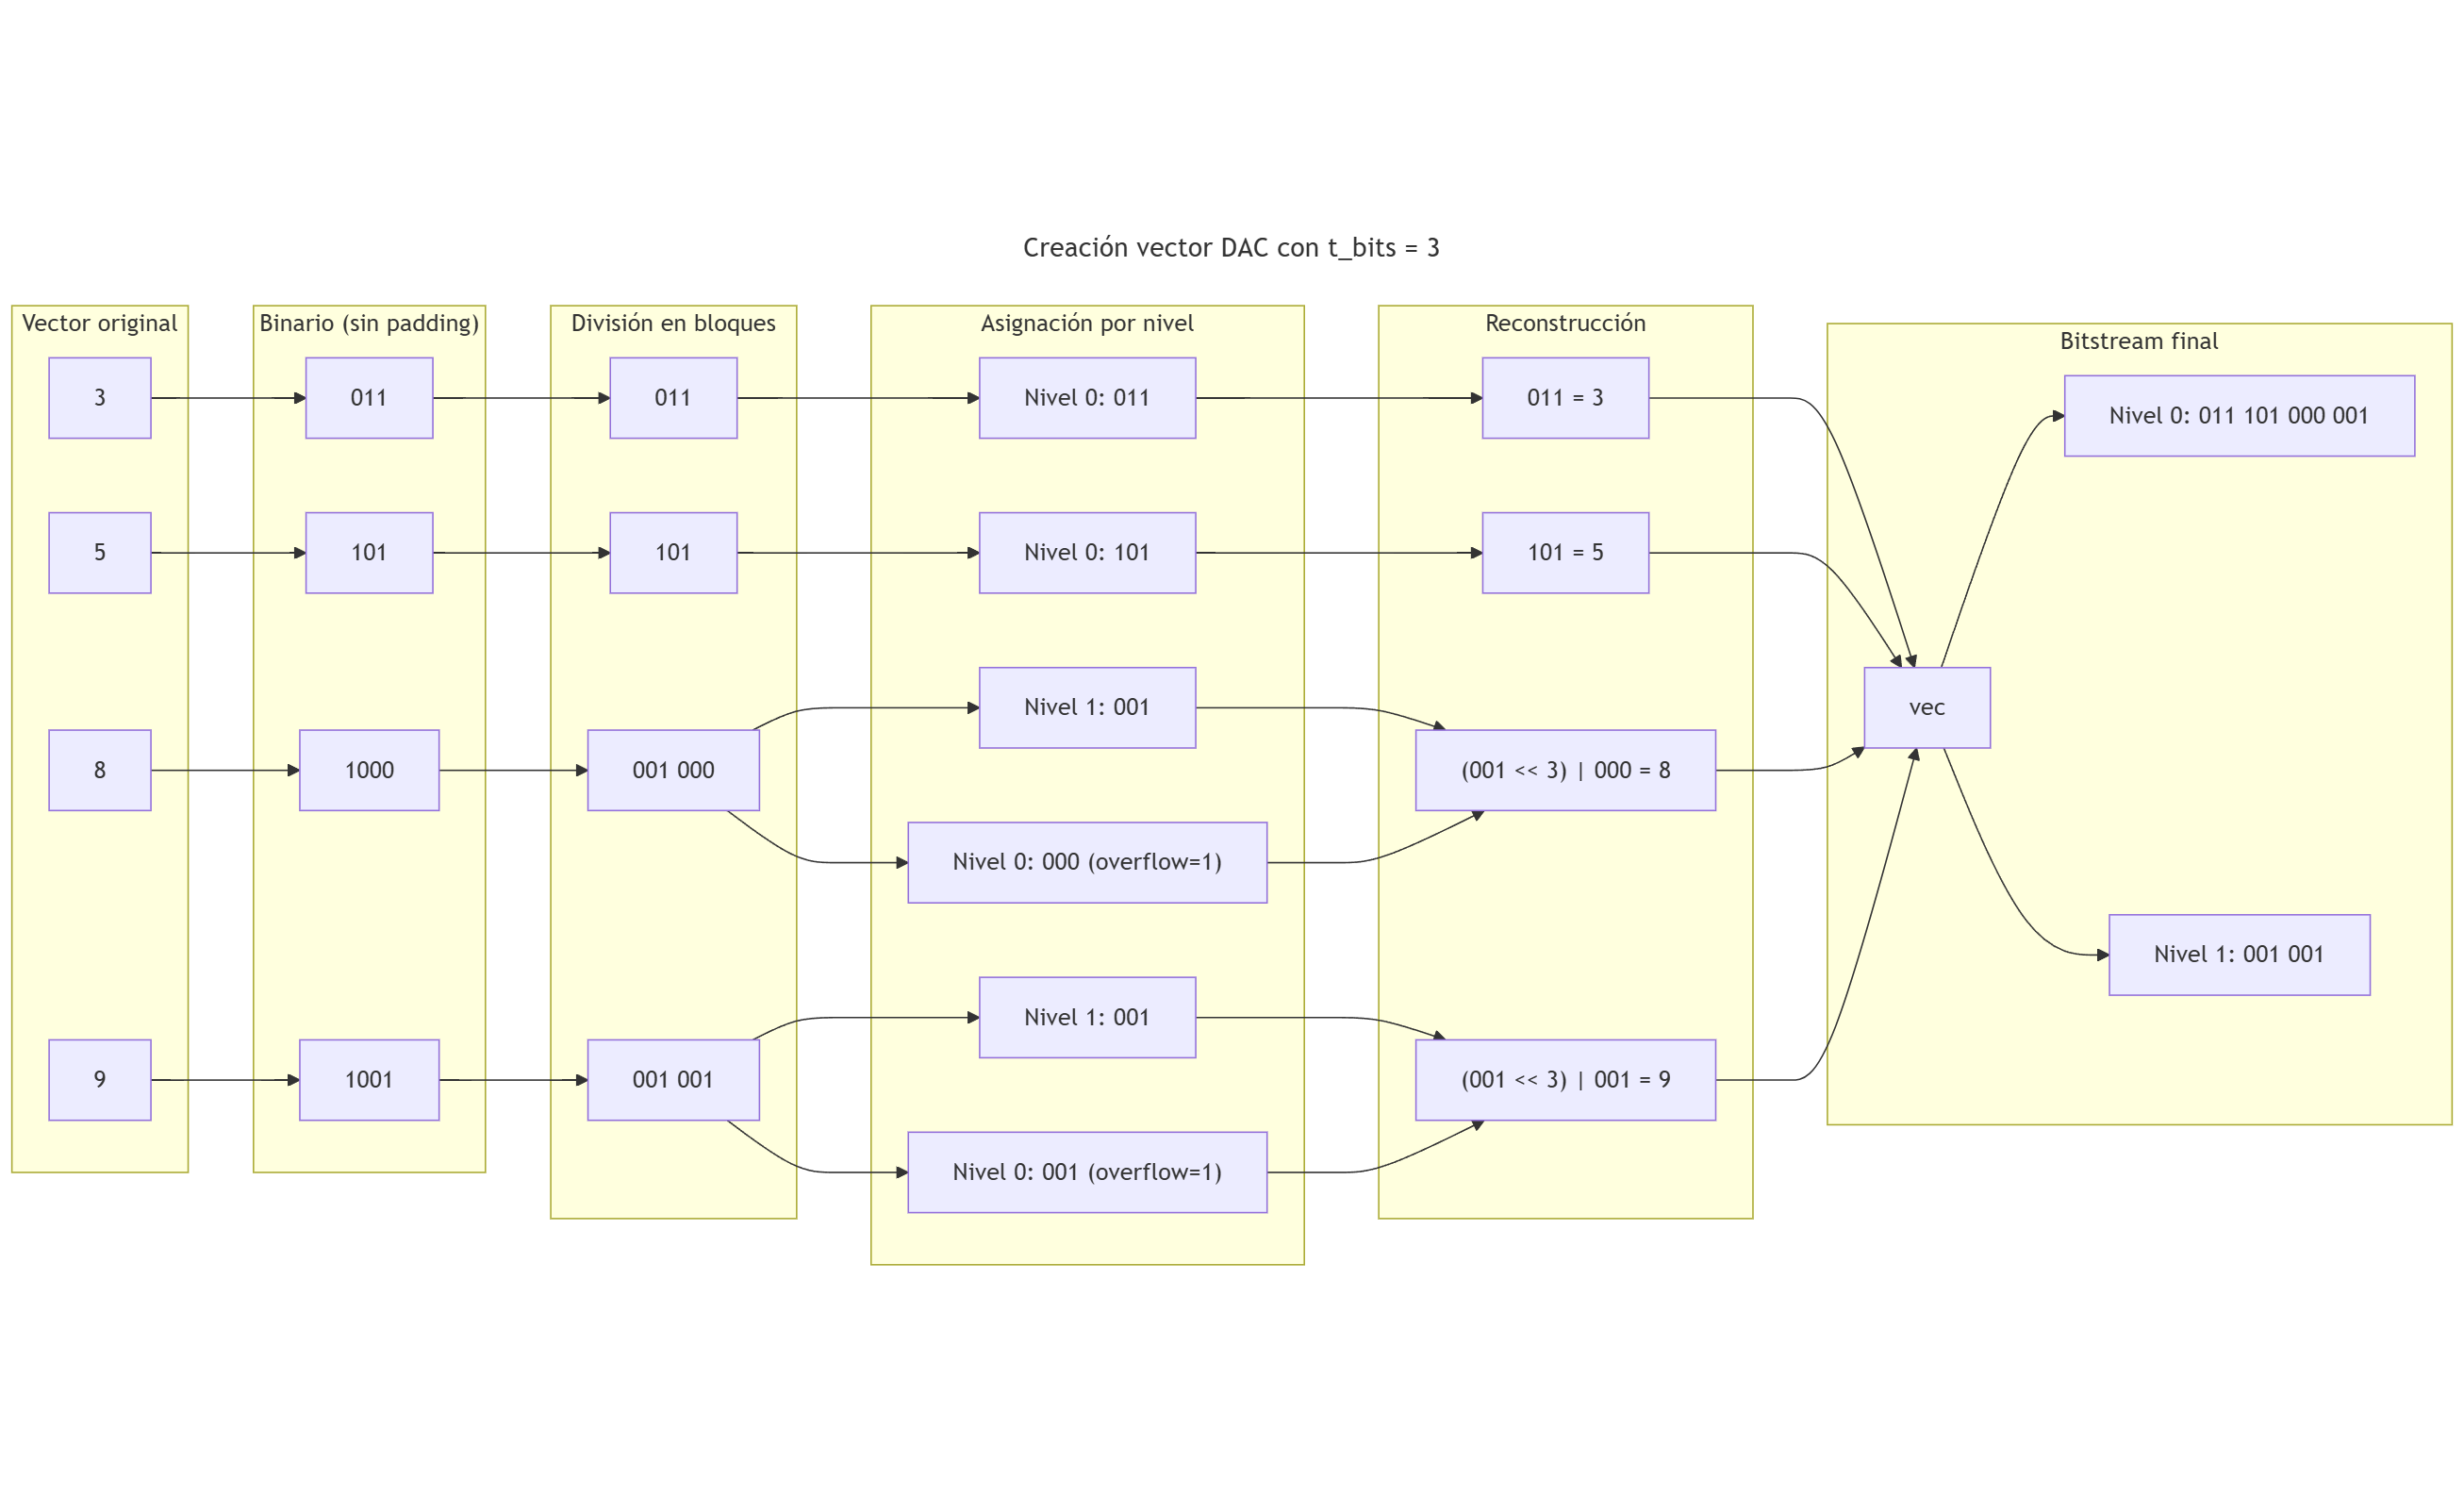
\includegraphics[width=1\textwidth]{alternatives/images/dac_vector.png}}
                \caption[Ejemplo \texttt{dac\_vector}]{Estructura escalonada del vector \texttt{dac\_vector}. Cada nivel almacena bloques de bits fijos con su correspondiente bit de continuación, permitiendo acceso eficiente sin necesidad de decodificar secuencialmente todo el vector.}
                \label{dac_vector}
            \end{figure}

            \item \textbf{Estructuras De Datos Compactas Disponibles}
            \begin{itemize}
                \item \texttt{enc\_vector\_<codificación>}:
                Almacena enteros codificados secuencialmente sin estructuras de acceso rápido.
                \begin{itemize}
                    \item \texttt{enc\_vector\_elias\_gamma}
                    \item \texttt{enc\_vector\_elias\_delta}
                    \item \texttt{enc\_vector\_fibonacci}
                    \item \texttt{enc\_vector\_comma\_2}
                \end{itemize}

                \item \texttt{vlc\_vector\_<codificación>}:
                Extiende a \texttt{enc\_vector} agregando muestreo para acceso eficiente.
                \begin{itemize}
                    \item \texttt{vlc\_vector\_elias\_gamma}
                    \item \texttt{vlc\_vector\_elias\_delta}
                    \item \texttt{vlc\_vector\_fibonacci}
                    \item \texttt{vlc\_vector\_comma\_2}
                \end{itemize}

                \item \texttt{dac\_vector}:
                Utiliza codificación escalonada por niveles con acceso eficiente directo.
            \end{itemize}
        \end{enumerate}
\end{enumerate}


Para evaluar estas estructuras de datos, se han medido tres métricas clave: el tiempo de acceso a los elementos, el tiempo de construcción de la estructura y el espacio utilizado en memoria. 

Es importante mencionar que debido a las limitantes de la implementación de \texttt{enc\_vector} dentro de la biblioteca \texttt{sdsl4py}, se ha omitido la estructura para su evaluación y posterior experimentación. 

\paragraph{Input}
\vspace{0.2cm}

Para garantizar una evaluación comprehensiva y representativa del comportamiento de las estructuras de datos comprimidas, se han diseñado cuatro tipos de vectores sintéticos que simulan diferentes patrones de datos comúnmente encontrados en aplicaciones reales:

\begin{enumerate}
    \item \textbf{Incremental pequeño (\texttt{incremental\_small}):} Vectores con valores crecientes que presentan pequeñas diferencias entre elementos consecutivos. Este patrón simula series temporales con crecimiento gradual o datos de sensores con variaciones mínimas. Los valores de $x$ siguen la secuencia $[1, 2, 3, ..., n]$, mientras que los valores de $y$ añaden una pequeña variación aleatoria en el rango $[0, 2]$ a cada posición.

    \item \textbf{Aleatorio (\texttt{random}):} Vectores con valores completamente aleatorios distribuidos uniformemente en un rango amplio. Este patrón representa el peor caso para algoritmos de compresión, ya que no presenta patrones predecibles. Tanto $x$ como $y$ contienen enteros aleatorios en el rango $[1, n \times 10]$.

    \item \textbf{Oscilante (\texttt{oscillating}):} Vectores que siguen un patrón de onda sinusoidal, alternando entre valores ascendentes y descendentes. Este comportamiento es típico en señales periódicas, datos de vibración o patrones cíclicos. Los valores de $x$ son secuenciales, mientras que $y$ sigue la función $y_i = \frac{n}{2}(1 + \sin(\frac{4\pi i}{n}))$.

    \item \textbf{Incremental grande (\texttt{incremental\_large}):} Vectores con valores crecientes que presentan grandes diferencias entre elementos consecutivos. Los valores de $x$ son secuenciales $[1, 2, 3, ..., n]$, y los valores de $y$ se calculan como $y_i = i \times \text{random}[50, 200]$.
\end{enumerate}

Cada vector de prueba contiene por defecto 10,000 elementos, proporcionando un volumen de datos suficiente para evaluar el rendimiento de las estructuras de datos compactas. Esta diversidad de patrones permite analizar cómo cada método de compresión se adapta a diferentes características de los datos, desde el caso ideal (datos con alta correlación) hasta el caso más desafiante (datos completamente aleatorios).

\paragraph{Resultados}
A continuación, se presenta un promedio de los resultados obtenidos al evaluar las distintas estructuras de datos compactas utilizando los vectores sintéticos mencionados anteriormente.

% añadir imagenes y tablas de resultados
\begin{figure}[H]
\centering
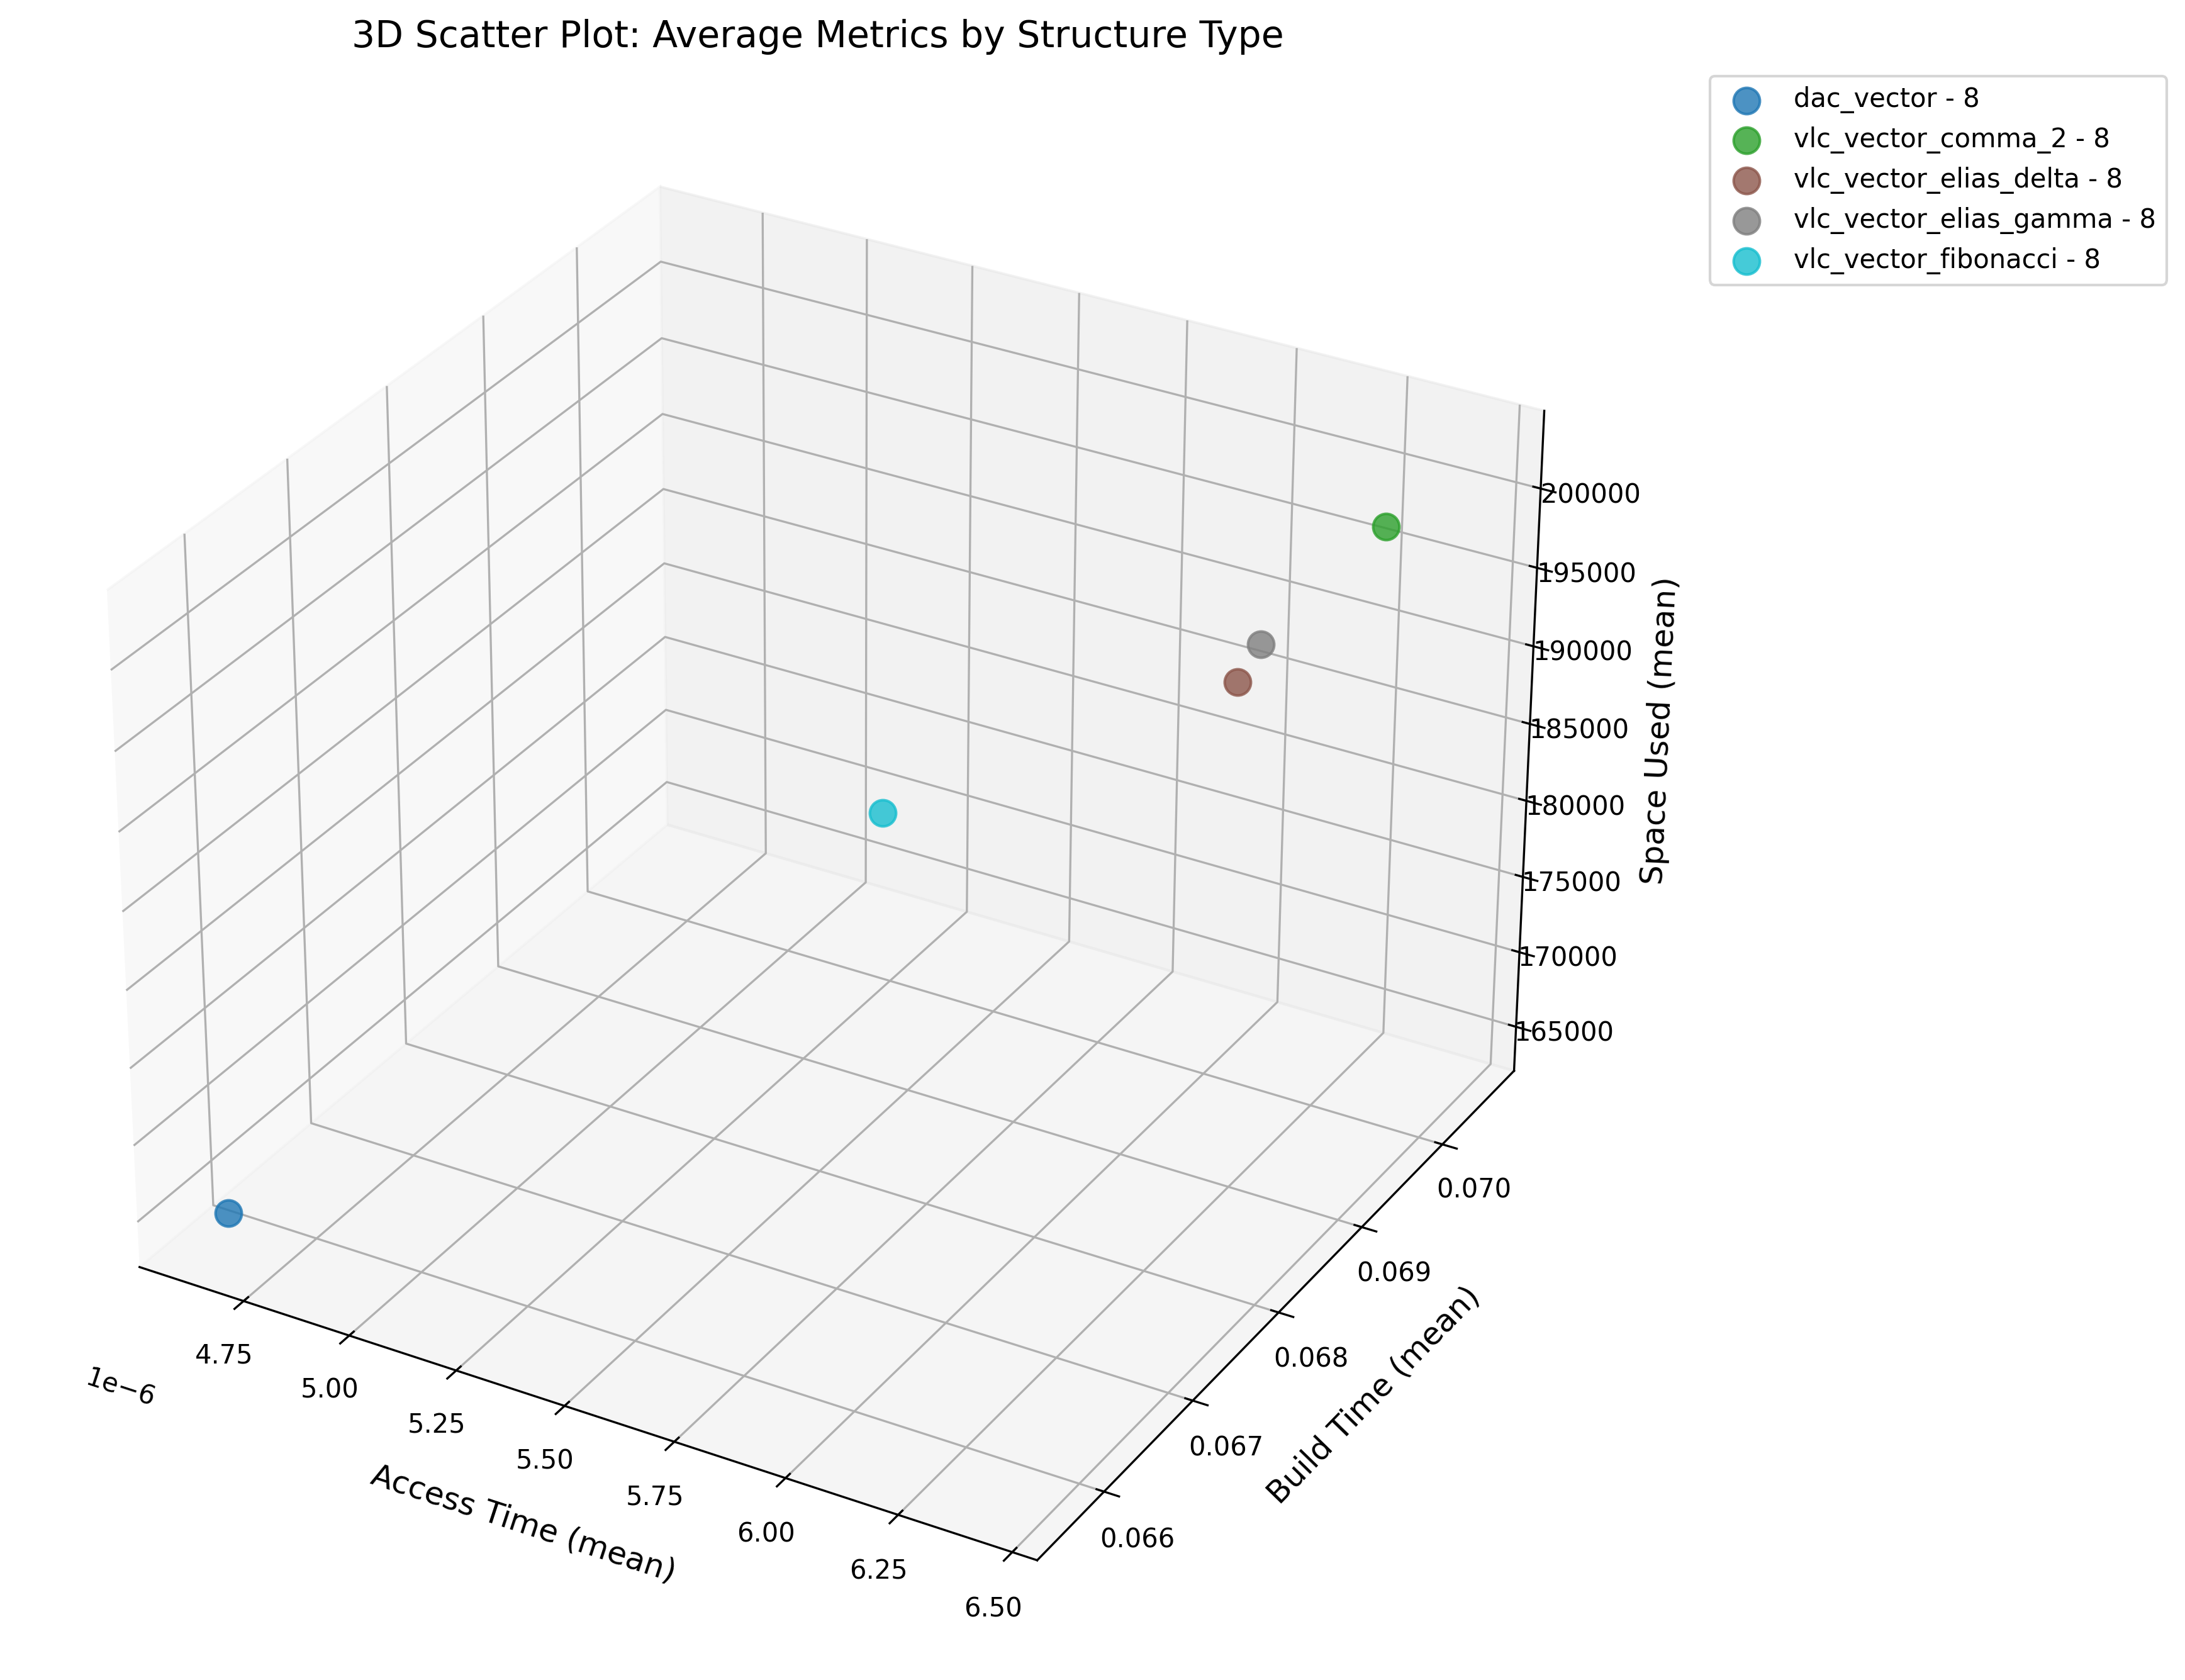
\includegraphics[width=0.8\textwidth]{alternatives/scatter_plot/3d_scatter_plot_structures.png}
\caption[Comparación Estructuras De Datos Compactas]{Puntajes promedio de las estructuras de datos compactas}   
\label{fig:scatter_plot_structures}
\end{figure}

\begin{figure}[H]
\centering
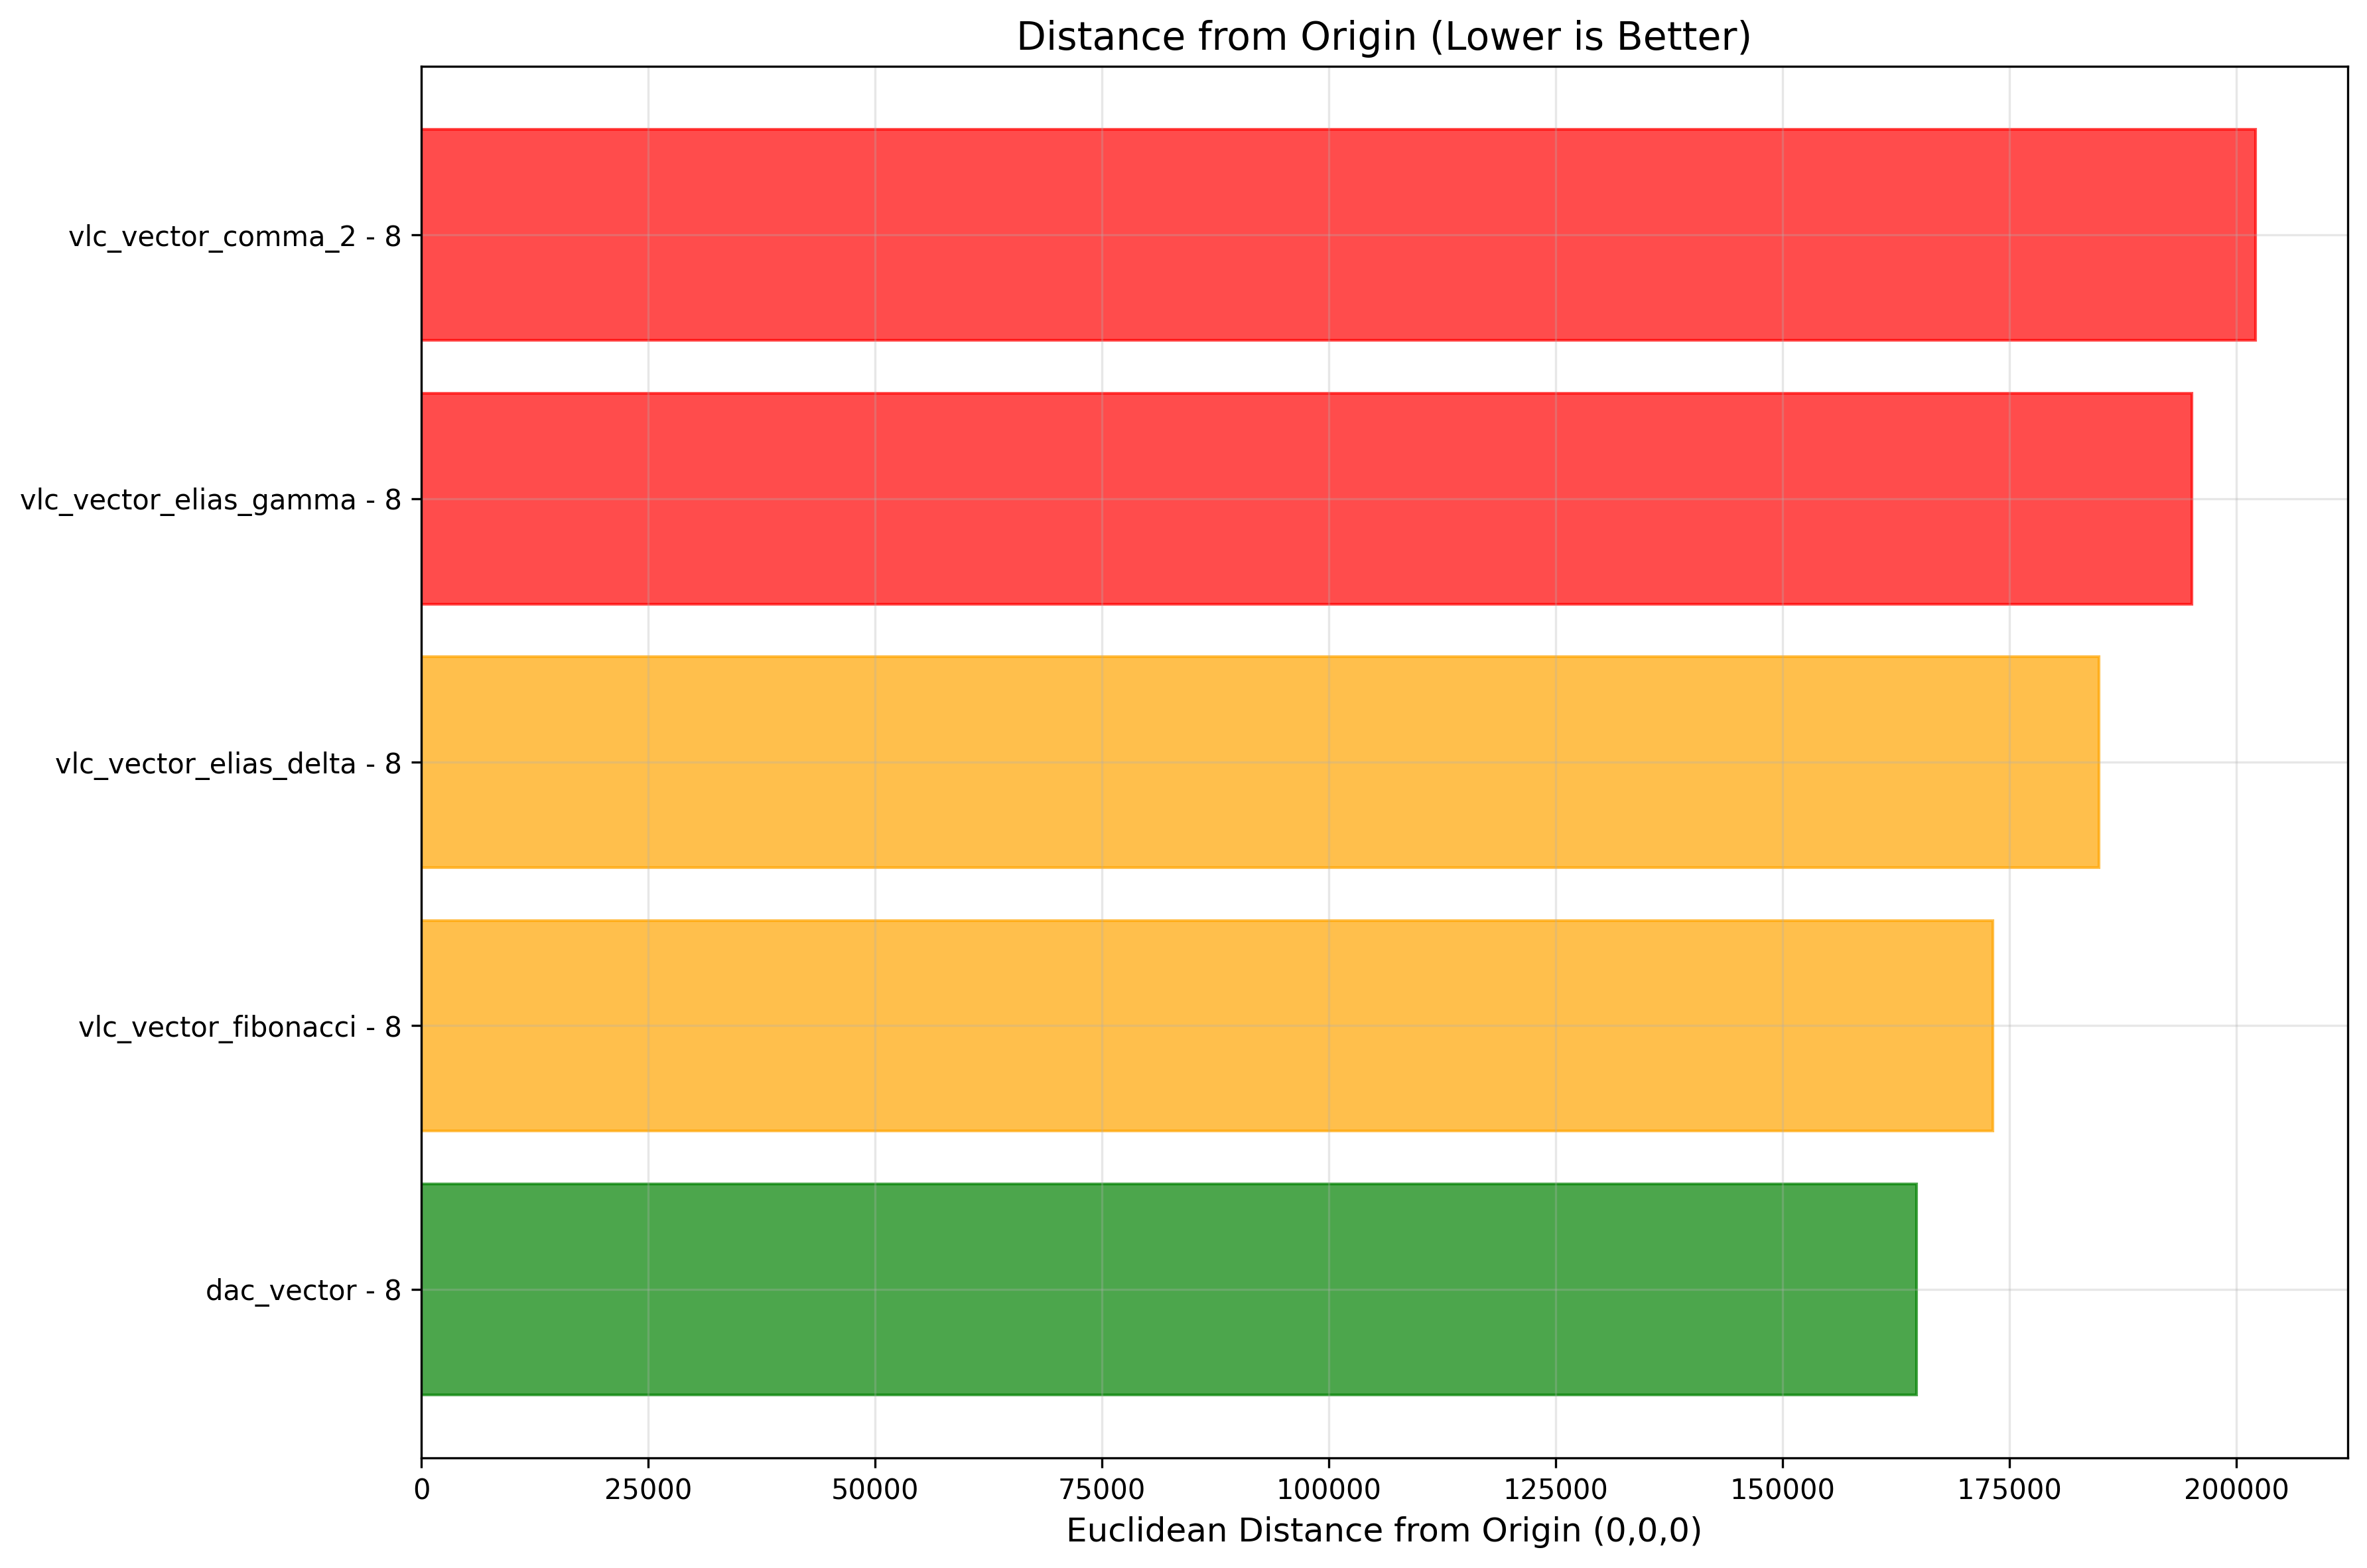
\includegraphics[width=0.8\textwidth]{alternatives/scatter_plot/euclidean_distance_from_ideal.png}
\caption[Distancia Euclidiana Estructuras De Datos]{Distancia euclidiana promedio de las estructuras de datos compactas respecto al punto $(0, 0, 0)$}   
\label{fig:euclidian_distance_from_ideal}
\end{figure}

\begin{table}[h!]
\centering
\caption[Comparación Estructuras de Datos Compactas]{RRanking de estructuras según su tiempo de acceso, tiempo de construcción y espacio usado.}
\label{tab:structure_ranking}
\begin{tabular}{|c|l|r|r|r|}
\hline
\textbf{Rank} & \textbf{Structure} & \textbf{Access} & \textbf{Build} & \textbf{Space} \\
\hline
1 & dac\_vector - 8 & 0.000005 & 0.065626 & 164749.3 \\
\hline
2 & vlc\_vector\_fibonacci - 8 & 0.000005 & 0.070020 & 173138.0 \\
\hline
3 & vlc\_vector\_elias\_delta - 8 & 0.000006 & 0.070556 & 184829.3 \\
\hline
4 & vlc\_vector\_elias\_gamma - 8 & 0.000006 & 0.069361 & 195058.7 \\
\hline
5 & vlc\_vector\_comma\_2 - 8 & 0.000006 & 0.069731 & 202126.7 \\
\hline
\end{tabular}
\end{table}


A partir de la puntuación resultante, se seleccionan las estructuras de datos \textit{dac\_vector} y \textit{vlc\_vector\_fibonacci} como las más adecuadas para el sistema, ya que son las que obtuvieron los puntajes más favorables en la evaluación.